% Created 2016-04-18 Mon 11:35
\documentclass[11pt]{article}
\usepackage[utf8]{inputenc}
\usepackage{lmodern}
\usepackage[T1]{fontenc}
\usepackage{fixltx2e}
\usepackage{graphicx}
\usepackage{longtable}
\usepackage{float}
\usepackage{wrapfig}
\usepackage{rotating}
\usepackage[normalem]{ulem}
\usepackage{amsmath}
\usepackage{textcomp}
\usepackage{marvosym}
\usepackage{wasysym}
\usepackage{amssymb}
\usepackage{amsmath}
\usepackage[version=3]{mhchem}
\usepackage[numbers,super,sort&compress]{natbib}
\usepackage{natmove}
\usepackage{url}
\usepackage{minted}
\usepackage{underscore}
\usepackage[linktocpage,pdfstartview=FitH,colorlinks,
linkcolor=blue,anchorcolor=blue,
citecolor=blue,filecolor=blue,menucolor=blue,urlcolor=blue]{hyperref}
\usepackage{attachfile}
\usepackage[left=1in, right=1in, top=1in, bottom=1in, nohead]{geometry}
\geometry{margin=1.0in}
\usepackage{amsmath}
\usepackage{siunitx}
\usepackage{graphicx}
\usepackage{epstopdf}
\usepackage{fancyhdr}
\usepackage{hyperref}
\usepackage[labelfont=bf]{caption}
\usepackage{setspace}
\usepackage{sectsty}
\subsectionfont{\rm}
\setlength{\headheight}{5.2pt}
\setlength{\headsep}{14pt}
\def\dbar{{\mathchar'26\mkern-12mu d}}
\pagestyle{fancy}
\fancyhf{}
\renewcommand{\headrulewidth}{0.5pt}
\renewcommand{\footrulewidth}{0.5pt}
\lfoot{\today}
\cfoot{\copyright\ 2016 W.\ F.\ Schneider}
\rfoot{\thepage}
\rhead{\bf{ND CBE 20255}}
\lhead{\bf{Quiz 3}}
\chead{\bf{Spring 2016}}
\setcounter{secnumdepth}{3}
\author{William F. Schneider}
\date{\today}
\title{CBE 60553 Outline}
\begin{document}

\begin{options}
\end{options}

\
\vspace{2cm}
\begin{figure}[h]
\centering

\includegraphics[width=0.4\textwidth]{../centered-2c-NDmark.pdf}
\end{figure}
\begin{center}
{\LARGE\bf Introduction to Chemical Engineering\\(CBE 20255)}
\vspace{0.5cm}

{\Large Prof. William F.\ Schneider}
\end{center}
\vspace{2cm}
\noindent\large{{\bf NAME (PRINT):}}\_\_\_\_\_\_\_\_\_\_\_\_\_\_\_\_\_\_\_\_\_\_\_\_\_\_\_\_\_\_\_\_\_\_\_\_\_\_

\vspace{1cm}
\begin{spacing}{1.2}
\begin{tabular}{|p{5.5in}|}
\hline
{\em AS A MEMBER OF THE NOTRE DAME COMMUNITY, I WILL NOT PARTICIPATE IN OR
TOLERATE ACADEMIC DISHONESTY } \\
\hline
\end{tabular}
\end{spacing}
\vspace{1.5cm}

\noindent\large{{\bf SIGNED:}} \_\_\_\_\_\_\_\_\_\_\_\_\_\_\_\_\_\_\_\_\_\_\_\_\_\_\_\_\_\_\_\_\_\_\_\_\_\_\_\_\_\_\_\_

\vspace{1cm}
\noindent{\bf PLEASE SHOW YOUR WORK.  CLEARLY DEMONSTRATE YOUR SOLUTION PROCEDURE
AND STATE ANY ASSUMPTIONS YOU MAKE.  WRITE YOUR SOLUTIONS IN THE SPACE
PROVIDED.  BLANK PAGES ARE INCLUDED TO PROVIDE MORE ROOM FOR YOUR
WORK.  ASK THE PROCTOR IF YOU NEED ADDITIONAL SCRATCH PAPER.}
\newpage


\section{Unsteamed}
\label{sec-1}
A \SI{10.0}{\meter\cubed} tank contains steam at \SI{275}{\celsius} and 15.0 bar.  You consult a steam table and find that the steam is superheated at this condition, with specific properties  \(\hat{V}=\SI{0.1610}{\meter\cubed\per\kilogram}\), \(\hat{U}=\SI{2741}{\kilo\joule\per\kilo\gram}\), \(\hat{H}=\SI{2982}{\kilo\joule\per\kilo\gram}\).  The tank and its contents are cooled until the pressure drops to \SI{1.8}{\bar}.  Some of the steam condenses in the process.

\begin{figure}[htb]
\centering
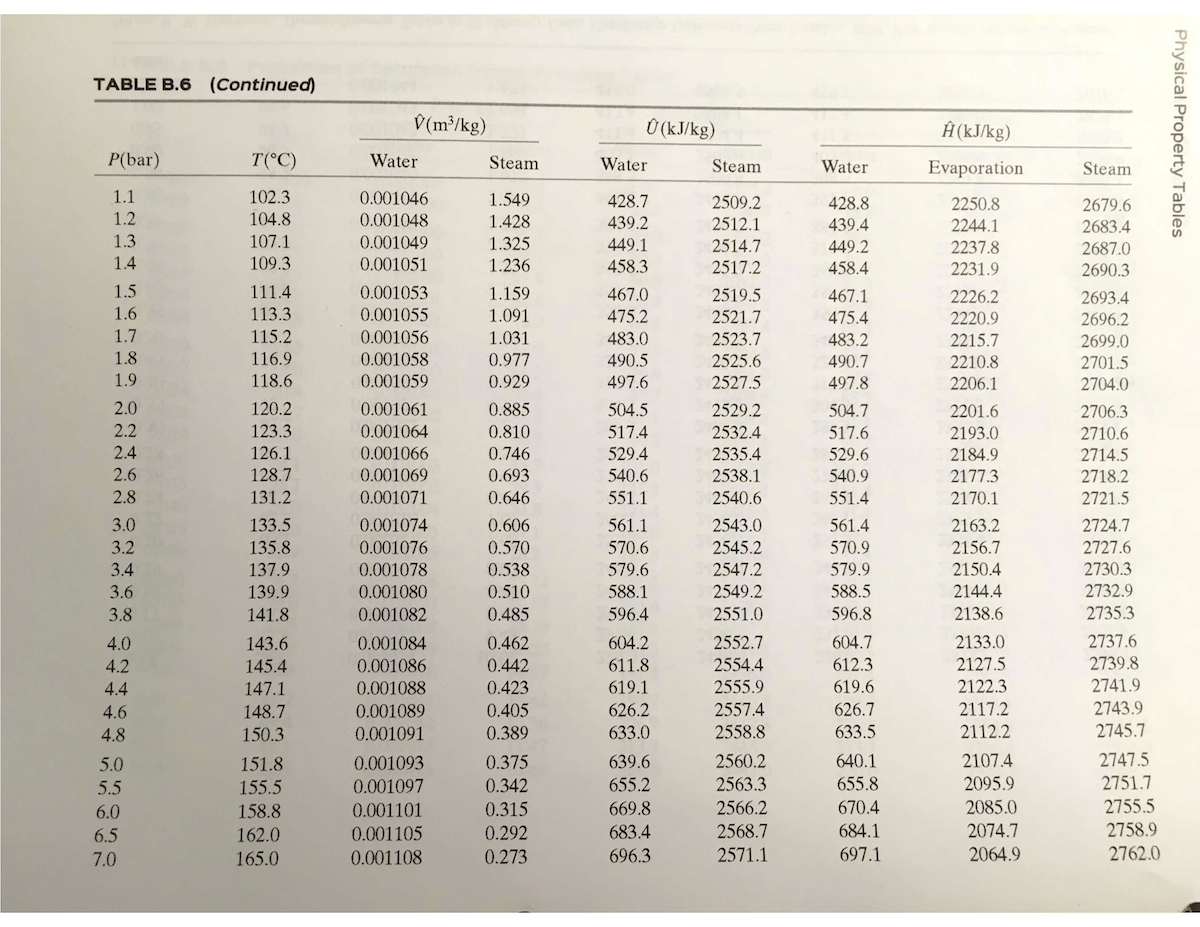
\includegraphics[width=0.8\textwidth]{./Quiz3.png}
\caption{A Fragment of a Saturated Steam Table}
\end{figure}

\subsection{(2 pts) What is the total mass (kg) of \ce{H2O} in the tank?}
\label{sec-1-1}
\newpage
\subsection{(2 pts) What is the final temperature of the tank contents?}
\label{sec-1-2}
\vspace{4cm}
\subsection{(4 pts) How much steam (kg) condensed?}
\label{sec-1-3}
\vspace{9cm}
\subsection{(4 pts) How much heat (kJ) was transferred from the tank?}
\label{sec-1-4}
\newpage


\section{Keep the water flowing}
\label{sec-2}
Water is to be delivered from an elevated reservoir into farm fields.  The water is to be delivered at a rate of \SI{4.00}{\meter\cubed\per\hour} through a pipe with cross-sectional area \SI{40}{\centi\meter\squared}, and the end of the pipe is \SI{300}{\meter} below the entrance.
\\

\noindent The Bernoulli equation might be helpful to remember:

\[\frac{1}{2}\Delta u^{2}+g \Delta z + \frac{1}{\rho}\Delta P = 0 \]

\subsection{(4 pts) What is the pressure difference between the exit and inlet of the pipe?}
\label{sec-2-1}
\vspace{10cm}
\subsection{(4 pts) How far below the surface of the reservoir is the pipe inlet?}
\label{sec-2-2}
% Emacs 25.0.50.1 (Org mode 8.2.10)
\end{document}